\documentclass[letterpaper]{article} % DO NOT CHANGE THIS
% --- Tectonic (XeTeX) draft builds only. aaai2027.sty calls \RequirePDFTeX and aborts on XeTeX.
% --- Inert under pdfLaTeX (\ifPDFTeX is true there). Delete this block (2 code lines) before the final submission.
\usepackage{iftex}
\ifPDFTeX\else\def\RequirePDFTeX{}\fi
% ---
% Public preprint build. For double-blind review, use \usepackage[submission]{aaai2027} and delete \nocopyright below.
\usepackage{aaai2027}
\usepackage[hyphens]{url}  % DO NOT CHANGE THIS
\usepackage{graphicx} % DO NOT CHANGE THIS
\urlstyle{rm} % DO NOT CHANGE THIS
\def\UrlFont{\rm}  % DO NOT CHANGE THIS
\usepackage{natbib}  % DO NOT CHANGE THIS AND DO NOT ADD ANY OPTIONS TO IT
\usepackage{caption} % DO NOT CHANGE THIS AND DO NOT ADD ANY OPTIONS TO IT
\frenchspacing  % DO NOT CHANGE THIS
\nocopyright % preprint only: no AAAI copyright notice (not allowed in AAAI-published papers)
\usepackage{booktabs}

\ifPDFTeX % \pdfinfo is a pdfTeX primitive; skipped in Tectonic draft builds
\pdfinfo{
/TemplateVersion (2027.1)
}
\fi

\setcounter{secnumdepth}{2}
\newcommand{\tbd}[1]{\textbf{[TBD: #1]}}

\title{Longer, Not Better: Rubric LLM Judges Favor Longer Forecasts, Not More Accurate Ones}
\author{Anonymous Authors}
\affiliations{}

\begin{document}

\maketitle

\begin{abstract}
LLM judges now score reasoning before any answer key exists, and their scores pick outputs, filter data and reward agents. We test such judges against reality. On 409 Kalshi questions that resolved in July--September 2026, after the stated training cutoffs of the forecasters and the primary judge, Claude Sonnet 5.5 and GPT-6 Luna each wrote 32 forecasts per question. Three pre-registered and two exploratory LLM judges scored all 26,176 forecasts with a published forecasting rubric. On Sonnet's forecasts, the primary judge's top-scored forecast scores like a random pick (Brier 0.246 against 0.248) and no better than always answering 50\% (0.250). Two rules that read no text do as well or better: the forecast nearest the mean of the 32 forecasts scores 0.242, and the mean shrunk toward 50\% scores 0.230. The market price, which no model saw, scores 0.192. Judge scores follow text length, not accuracy: of two forecasts written from the same evidence, the judge prefers the longer one 55\% of the time and the more accurate one 50\%. When only the stated probability changes, judges penalize extremizing it more than shrinking it, although only shrinking improves accuracy. We propose two audits of judges that need no outcomes.
\end{abstract}

\section{Introduction}
Large language models now act as judges where no answer key exists yet. A judge reads a model's reasoning, scores it against a rubric, and the system keeps the best-scored output. Best-of-$N$ sampling, data filtering and rubric rewards for reinforcement learning \citep{gunjal2025rubrics,viswanathan2025checklists}, now also for forecasting agents \citep{anonymous2026beliefstate}, all assume that a higher rubric score means a better answer. The assumption is hard to test, because the truth is unknown when the judge scores. It matters most for outputs that only reality can grade, such as the forecasts and research claims of AI agents.

Forecasting lets us test it. A forecast can be judged today and scored against the outcome later. We ask: \emph{given many forecasts of the same event by the same model, does an outcome-blind rubric judge prefer the more accurate ones?}

We use 409 prediction-market questions that resolved after the stated training cutoffs of the forecasters and the primary judge. Two forecasters each wrote 32 forecasts per question from subsets of the same news. Five judges scored every forecast with the Prophet Arena rubric \citep{prophetarena2025}. We fixed four endpoints before the run.

The answer is no. The judge's pick scores like a random pick, and two simple rules that read only the stated probabilities do as well or better (Section~\ref{sec:pick}). Judge scores follow the length of the reasoning, not its accuracy (Section~\ref{sec:length}). With the text held fixed, the stated number alone moves the score (Section~\ref{sec:edits}). The picture is similar for five judges, two scoring scales and, with a wide interval, a stronger judge on a pilot subset.

Our contributions are: (1) a pre-registered test of rubric-based selection against resolved outcomes, on 26,176 forecasts; (2) two audits of a judge that need no outcomes, a same-evidence pair test and a number-edit test; (3) a practical rule for forecasting pipelines: average the forecasts and shrink the average toward 50\%, instead of selecting one with a rubric judge.

\section{Related Work}
\paragraph{Judge biases.} LLM judges prefer longer answers \citep{zheng2023judging,saito2023verbosity,dubois2024length} and their own outputs \citep{panickssery2024llm}. Reward-model scores track length \citep{singhal2023long} and favor answers that state high confidence \citep{leng2025taming}. Without a correct reference answer, judges score plausibility rather than correctness \citep{krumdick2025nofree,zhou2026more}. Pairs of responses with the same content can expose such biases without labels \citep{labelfree2026}. These studies measure bias against human labels or known answers; we measure it against outcomes that nobody knew when the judge scored.

\paragraph{Best-of-$N$ with imperfect verifiers.} Trained verifiers make best-of-$N$ work in math \citep{cobbe2021training,lightman2024lets}. Optimizing too hard against an imperfect proxy reward lowers the true reward \citep{gao2023scaling}, and false positives cap what resampling can gain \citep{stroebl2024inference}. On 5,000 Chatbot Arena prompts, a judge's best-of-4 pick captures 21\% of the gain of a perfect pick \citep{landesberg2026}.

\paragraph{Judging forecasts.} LLM forecasters approach human crowds \citep{halawi2024approaching,schoenegger2024wisdom} but still trail experts \citep{karger2025forecastbench}. In the AIA Forecaster, an LLM's best-of-10 pick scores worse than the mean of the 10 \citep{aia2025forecaster}; that study tests one $N$ and no rubric. LLM ratings of human rationales correlate 0.19 with relative accuracy \citep{fri2026}, and text features of rationales correlate modestly with forecaster skill \citep{karvetski2022forecasting}. Dropping forecasts whose reasoning contradicts their stated number improves accuracy \citep{gorur2025argumentatively}. Prophet Arena's rubric, which we use, compares models and agrees with human raters \citep{prophetarena2025}, and outcome-blind rubric scores track skill across seven models \citep{echo2026}. No study tests whether a rubric can rank one model's own forecasts against outcomes. Our shrunk mean resembles the one-parameter logit aggregator of \citet{satopaa2014combining}. Aggregates of independent forecasters usually need extremizing \citep{baron2014two}, but our pools come from one overconfident model, so our factor shrinks.

\section{Setup}\label{sec:setup}
\paragraph{Questions.} We start from Prophet-Arena-Subset-3000, a public set of Kalshi markets with news sources collected at a fixed snapshot time \citep{prophetarena2025}. We keep the markets whose snapshot and close both fall on or after July 1, 2026, after the stated training cutoffs of the forecasters and the primary judge (June 2026 or earlier). We also require a horizon of 12 hours or more, a mid price of 5--95 cents, a spread of 10 cents or less and two markets or fewer per event, and drop sports. This leaves 409 markets from 228 events in ten categories. They closed between July 3 and September 7, 2026 (median horizon 4.6 days), and 46.7\% resolved YES. Each question has a median of 10 sources (title, link and summary). We delete every sentence that quotes a market price, betting odds or a model probability.

\paragraph{Forecasters.} Claude Sonnet 5.5 (default settings, including its built-in thinking, which 88\% of forecasts used) and GPT-6 Luna (reasoning effort `none', temperature 1) write step-by-step reasoning that ends with ``FINAL PROBABILITY: 0.xx''. For each question we draw 8 fixed subsets of the sources, each with half of them and at least 3. Both forecasters see the same subsets, and each writes 4 forecasts per subset: 32 forecasts per forecaster and question, 26,176 in all. A Sonnet text has a median of 256 words and a Luna text 179. Within a question, the stated probabilities have a median standard deviation of 0.048 (Sonnet) and 0.076 (Luna).

\paragraph{Judges.} Judges use the Prophet Arena reasoning rubric: five criteria (sources, evidence, synthesis, uncertainty, and how well the probability follows from the reasoning), each scored 1--5, for a total of 5--25. The judge sees the question and its resolution rules, the titles and links of the sources the forecaster saw, and the forecast's text with its probability. It is told that it does not know the outcome. A forecast's score is the mean over repeated calls. The primary judge is Claude Haiku 5.5 (5 repeats). Gemma 4 31B and GLM-5 (3 repeats each) passed a gate fixed before the run (Appendix~\ref{app:gate}); with Haiku they are the three \emph{pre-registered judges}. Gemini 3.1 Flash-Lite and DeepSeek V4 Flash failed the gate and serve as exploratory judges. Haiku also scored every forecast on a 1--10 version of the rubric, and GPT-5.5 scored a 150-question pilot with 16 forecasts per question. In leak probes, no judge stated a July--September 2026 outcome (Appendix~\ref{app:gate}; GPT-5.5 was not probed), and the forecasters' accuracy shows no sign of outcome knowledge (Section~\ref{sec:pick}).

\paragraph{Selection and baselines.} For each question and each $N \in \{1, 2, 4, 8, 16, 32\}$, we draw $N$ of the 32 forecasts 200 times. The \emph{judge pick} $J$ is the top-scored forecast, with ties broken at random. We score forecasts with the Brier score $(p - y)^2$ \citep{brier1950verification}: lower is better, and always answering 50\% gives 0.25. We compare $J$ with four baselines. The \emph{random pick} $R$ is the mean Brier score of the $N$ forecasts. The \emph{plain mean} $M$ forecasts their mean probability. The \emph{shrunk mean} $S$ forecasts the same mean after multiplying its log-odds by one factor fitted on other events (five folds by event). The \emph{best pick in hindsight} $O$ is the most accurate of the $N$ forecasts. The \emph{hindsight gain} is $R - O$, and \emph{recovery}, $(R - J)/(R - O)$, is the share of it that the judge captures.

\paragraph{Two audits without outcomes.} \emph{Same-evidence pairs:} two forecasts from the same source subset saw the same evidence. For each such pair (48 per question and forecaster, ties dropped) we ask whether the judge prefers the more accurate forecast and whether it prefers the longer one. \emph{Number edits:} we keep a forecast's text and change only its probability in log-odds, shrinking it ($\times 0.5$) or extremizing it ($\times 2$); an unedited control is rebuilt the same way. In \emph{number-only} edits the text never states the number, so the final line is the only change (478 Sonnet and 382 Luna forecasts). In \emph{text-and-number} edits every copy of the number changes (255 and 405 forecasts).

\paragraph{Statistics and pre-registration.} Confidence intervals resample events (2,000 bootstrap draws), because questions from one event are correlated. Before the run we fixed four endpoints for the primary combination, Haiku judging Sonnet. Appendix~\ref{app:changes} lists every change to the plan.\newline
\textbf{E1:} the judge pick is worse than the shrunk mean at $N = 32$.\newline
\textbf{E2:} the upper 95\% bound of recovery at $N = 32$ is below 20\%.\newline
\textbf{E3:} the judge prefers the more accurate forecast of a pair $50\% \pm 2$ points of the time (two one-sided tests \citep{schuirmann1987comparison}, 90\% interval), and the longer one more than half the time.\newline
\textbf{E4:} extremizing costs more score than shrinking, and the cost does not depend on whether the edit moves the number toward the realized outcome (the \emph{direction test}).

\section{Results}\label{sec:results}

\begin{figure}[t]
\centering
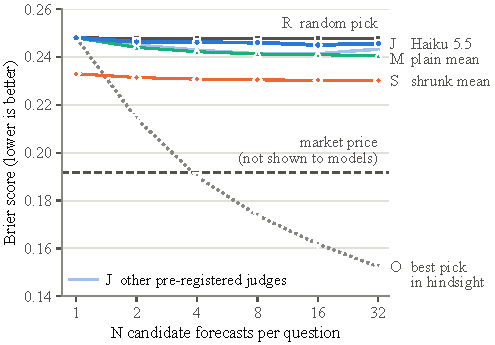
\includegraphics[width=\columnwidth]{figures/fig1_brier_vs_n.pdf}
\caption{Brier score (lower is better) against the number $N$ of candidate forecasts, Claude Sonnet 5.5. The judge's pick ($J$, Haiku thick; the other pre-registered judges thin) stays at the random pick $R$ while the best pick in hindsight $O$ improves. The plain mean $M$ is as good as the pick, and the shrunk mean $S$ is better. The dashed line is the market price, which no model saw.}
\label{fig:curves}
\end{figure}

\subsection{The judge's pick scores like a random pick}\label{sec:pick}
In Figure~\ref{fig:curves} (Sonnet), the best pick in hindsight improves fast, from 0.248 at $N = 1$ to 0.152 at $N = 32$. The judge's pick stays near the random pick. At $N = 32$, Haiku's pick scores 0.246 against 0.248 for a random pick (difference $-0.002$, 95\% CI $-0.013$ to $0.008$). It recovers 2\% of the hindsight gain ($-9\%$ to $13\%$), so E2 holds. For the three pre-registered judges on both forecasters, recovery is 0--5\%, and every upper bound is below 15\% (Table~\ref{tab:cells} in the appendix).

The best pick in hindsight mostly picks luck (an exploratory check). We replaced each question's 32 forecasts with 32 random draws that have the same mean and spread in log-odds but carry no information. The best of these draws scores 0.145 on Sonnet and 0.118 on Luna, close to the real 0.152 and 0.120. Noise of this size yields the whole hindsight gain, so recovery is a weak yardstick, and Table~\ref{tab:ladder} compares Brier scores directly.

A single forecast is no better than a constant: a random pick scores 0.248 (Sonnet) and 0.259 (Luna), against 0.250 for always answering 50\%. Two simple rules that look only at the 32 probabilities beat a random pick (exploratory). On Sonnet, the forecast nearest the mean of the 32 scores 0.242, and the least extreme forecast scores 0.233. Haiku reads about 8,000 words of reasoning per question, and its pick scores 0.246; taking the longest text scores 0.243. The two rules match the judge's pick on Sonnet and beat it on Luna (least extreme: by 0.022, 0.006 to 0.038, pooled over the pre-registered judges). The plain mean scores 0.241. The shrunk mean scores 0.230 and beats the judge's pick by 0.015 (0.001 to 0.031), so E1 holds. Both forecasters are overconfident (the best shrink factors are about 0.45 and 0.40), which is also why the least extreme forecast does well. The market price, which no model saw, scores 0.192.

\begin{table}[t]
\centering
\small
\begin{tabular}{@{}lll@{}}
\toprule
Option at $N = 32$ & Sonnet & Luna \\
\midrule
\multicolumn{3}{@{}l}{\emph{No information}} \\
\quad Always 50\% & 0.250 & 0.250 \\
\quad Always the base rate (46.7\%) & 0.249 & 0.249 \\
\multicolumn{3}{@{}l}{\emph{Pick one of the 32 by a simple rule}} \\
\quad Most extreme & 0.279 & 0.308 \\
\quad Random & 0.248 & 0.259 \\
\quad Longest text & 0.243 & 0.252 \\
\quad Nearest the mean of the 32 & 0.242 & 0.246 \\
\quad Least extreme & 0.233 & 0.235 \\
\multicolumn{3}{@{}l}{\emph{Pick the judge's top-scored forecast (recovery)}} \\
\quad Haiku 5.5 & 0.246 (2\%) & 0.257 (1\%) \\
\quad Gemma 4 31B & 0.243 (5\%) & 0.258 (0\%) \\
\quad GLM-5 & 0.243 (5\%) & 0.254 (3\%) \\
\multicolumn{3}{@{}l}{\emph{Combine the 32}} \\
\quad Plain mean & 0.241 & 0.246 \\
\quad Shrunk mean & 0.230 & 0.234 \\
\multicolumn{3}{@{}l}{\emph{Use what no model saw}} \\
\quad Nearest the market price & 0.213 & 0.207 \\
\quad Market price & 0.192 & 0.192 \\
\quad Best pick in hindsight & 0.152 & 0.120 \\
\bottomrule
\end{tabular}
\caption{Brier score at $N = 32$ (lower is better) on 409 questions. Recovery is the share of the hindsight gain that a pick captures; CIs for the judge rows are in Table~\ref{tab:cells}. The base-rate row, the simple rules and the market rows are exploratory.}
\label{tab:ladder}
\end{table}

\subsection{Scores follow length, not accuracy}\label{sec:length}
Within a question, the scores of the pre-registered judges correlate with the length of the text (Spearman 0.14 to 0.34) but hardly with accuracy (0.00 to 0.04). Figure~\ref{fig:pairs}a shows the same-evidence pairs. On Sonnet pairs, Haiku prefers the more accurate forecast 50.3\% of the time (90\% interval 49.4--51.2\%, 13,959 pairs). Within the pre-registered margin of $\pm 2$ points, its preference is independent of which forecast is more accurate, so E3 holds. Equivalence fails narrowly for Gemma on Sonnet (51.1\%) and Haiku on Luna (48.6\%), just above and just below chance. Haiku prefers the longer forecast 54.6\% of the time, and across the ten judge--forecaster combinations the longer one wins 53--66\% of pairs. On average, the forecast Haiku prefers has a Brier score 0.0004 higher than the other one ($-0.0010$ to $0.0020$; exploratory); in all ten combinations this gap lies between $-0.0022$ and $+0.0015$, and every CI includes zero. Length does not predict accuracy either: the longer forecast is the more accurate one in 49\% of pairs (exploratory).

These shares hide one effect. When both forecasts of a pair lean the same way, the more extreme one (the one farther from 50\%) is the more accurate one 63\% (Sonnet) and 62\% (Luna) of the time, because the forecasters usually get the direction right. A judge could thus win most pairs just by favoring confident forecasts, although this would worsen the Brier score. Three exploratory checks remove the effect. First, in the 5\% of Sonnet pairs that disagree on the direction, Haiku prefers the forecast on the right side 49.5\% of the time (44.9\% to 54.4\%). Second, in pairs that agree, Haiku prefers the more extreme forecast 52.0\% of the time when the shared direction turns out right, and 51.8\% when it turns out wrong. Third, a linear model of the judge's preference holds length and extremity fixed. In it, being the more accurate forecast raises the chance of being preferred by 0.0 percentage points ($-1.0$ to $1.0$), while 100 extra words raise it by 18 points (15 to 21). In all ten combinations the accuracy term lies between $-1.1$ and $+0.7$ points, and every CI includes zero.

\begin{figure*}[t]
\centering
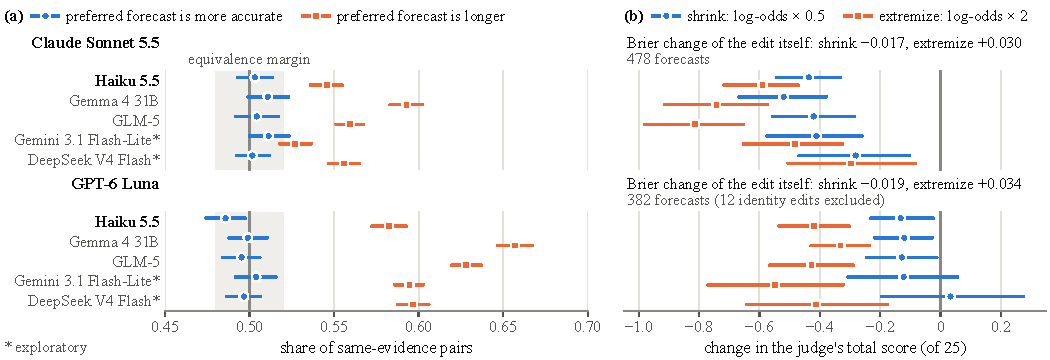
\includegraphics[width=\textwidth]{figures/fig2_pairs_edits.pdf}
\caption{(a) Same-evidence pairs: the share of pairs in which the judge's preferred forecast is the more accurate one (circles) and the longer one (squares), with 95\% CIs. The band marks the pre-registered equivalence margin of 48--52\% (the test itself uses 90\% intervals). (b) Number-only edits, rows as in (a): the change in the judge's total score (of 25), with 95\% CIs, when only the stated probability is shrunk (log-odds $\times 0.5$) or extremized ($\times 2$). $^*$Exploratory judges that failed the gate.}
\label{fig:pairs}
\end{figure*}

\subsection{The stated number alone moves the score}\label{sec:edits}
Number edits hold the text fixed (Figure~\ref{fig:pairs}b). In number-only edits of Sonnet forecasts, Haiku lowers its score by 0.44 (of 25) when the number is shrunk and by 0.59 when it is extremized. The difference, $-0.15$ ($-0.26$ to $-0.05$), supports E4. On Luna the costs are 0.13 and 0.42. In number-only edits, extremizing costs more than shrinking for all ten judge--forecaster combinations, significantly for eight, including all six with pre-registered judges. In text-and-number edits of Sonnet forecasts, the difference is $+0.05$ ($-0.11$ to $0.21$): there, shrinking and extremizing cost about the same. Pooled over both kinds of edit, the Sonnet difference is not significant ($-0.08$, $-0.18$ to $0.01$), so for the primary combination E4 holds only for number-only edits.

The rubric asks whether the number follows from the reasoning, so any edit should cost. It does not say that a move away from 50\% should cost more, nor that a move toward the judge's own forecast should cost less. Both happen. Shrinking made these forecasts more accurate (Brier $-0.017$ on Sonnet, $-0.019$ on Luna) and extremizing made them less accurate ($+0.030$, $+0.034$). For Haiku, the cost does not follow the realized outcome: none of its direction tests is significant. Of 36 overlapping tests for the pre-registered judges, 3 are; two concern GLM-5 on shrunk Sonnet forecasts, where the direction test fails (pooled $+0.33$, $0.12$ to $0.54$). In an exploratory test, edits that move the number toward the judge's own forecast of the question cost less: 11 of 60 overlapping tests are significant, all in this direction.

\subsection{Robustness}
The results hold on a 1--10 version of the rubric (Haiku recovers 3\% on Sonnet and 4\% on Luna) and for the two judges that failed the gate (Table~\ref{tab:cells}). This matters because the gate chose the secondary judges partly for agreeing with Haiku; the two failed judges were not chosen that way. The noisier of them, DeepSeek V4 Flash, beats a random pick on Sonnet by 0.008 (0.001 to 0.017), but not a randomly chosen forecast at the same distance from 50\% (difference $-0.0004$, $-0.004$ to $0.003$). On a 150-question pilot with 16 forecasts per question, GPT-5.5 recovers 10\% ($-5\%$ to $24\%$), against 5\% for Haiku on the same forecasts.

\section{Discussion}
\paragraph{What the judges reward.} The judges reward visible effort, such as a longer text, and grade the stated number by its distance from 50\% and, tentatively, from their own belief. None of this tracks accuracy here. As a reward, such a rubric is unlikely to teach a model to forecast better, though we did not train any model.

\paragraph{Then trust what?} Trust the pool, not a picker. The plain mean scores at least as well as the judge's pick. Shrinking toward 50\% does better still, whether by one factor fitted on resolved questions or by simply taking the least extreme forecast. Only rules that use the market price beat the shrunk mean. Whether humans pick better is untested.

\paragraph{Limitations.} Our forecasters are weak on these questions: a single forecast is no better than a constant, and the 32 forecasts of a question differ mostly by noise. A judge might do better on pools with real quality differences, such as forecasts from different models. Even so, the judges did not just miss a small signal: they rewarded length and the stated number. We used one rubric, the judge saw source titles but not texts, and the questions are short-horizon Kalshi markets without sports. The length evidence is correlational: we did not pad texts.

\section{Conclusion}
On 409 resolved questions, outcome-blind rubric judges picked among 32 forecasts about as well as a random pick. Their scores followed length and the stated number, not accuracy, and a simple shrunk mean did better than every judge's pick. Judge-based selection and rubric rewards for forecasting should be checked against outcomes before they are trusted. Before outcomes arrive, a judge should at least pass our two audits: it should not prefer the longer of two same-evidence forecasts, nor penalize extremizing more than shrinking.

\bibliography{references}

\appendix

\begin{table*}[t]
\centering
\footnotesize
\setlength{\tabcolsep}{4pt}
\begin{tabular}{@{}lccccc@{}}
\toprule
Judge & Recovery (\%) & $J - R$ & $J - S$ & Pairs: more accurate & Pairs: longer \\
\midrule
\multicolumn{6}{@{}l}{\emph{Forecaster: Claude Sonnet 5.5}} \\
Haiku 5.5 & 2 [$-$9, 13] & $-$0.002 [$-$0.013, 0.008] & 0.015 [0.001, 0.031] & 0.503 [0.494, 0.512] & 0.546 [0.536, 0.555] \\
Gemma 4 31B & 5 [$-$5, 14] & $-$0.004 [$-$0.013, 0.005] & 0.013 [$-$0.0004, 0.028] & 0.511 [0.501, 0.521] & 0.593 [0.583, 0.602] \\
GLM-5 & 5 [$-$4, 14] & $-$0.005 [$-$0.013, 0.004] & 0.013 [$-$0.0004, 0.026] & 0.504 [0.494, 0.515] & 0.560 [0.551, 0.568] \\
3 pre-registered, avg. & 4 [$-$5, 13] & $-$0.004 [$-$0.012, 0.005] & 0.014 [0.001, 0.028] & -- & -- \\
Haiku 5.5, 1--10 scale & 3 [$-$7, 12] & $-$0.003 [$-$0.012, 0.006] & 0.015 [0.001, 0.029] & 0.502 [0.493, 0.511] & 0.571 [0.563, 0.580] \\
Gemini 3.1 Flash-Lite$^*$ & 2 [$-$8, 12] & $-$0.002 [$-$0.011, 0.007] & 0.016 [0.001, 0.030] & 0.511 [0.502, 0.521] & 0.527 [0.518, 0.536] \\
DeepSeek V4 Flash$^*$ & 9 [1, 17] & $-$0.008 [$-$0.017, $-$0.001] & 0.009 [$-$0.003, 0.023] & 0.502 [0.493, 0.510] & 0.556 [0.547, 0.565] \\
\midrule
\multicolumn{6}{@{}l}{\emph{Forecaster: GPT-6 Luna}} \\
Haiku 5.5 & 1 [$-$7, 9] & $-$0.001 [$-$0.013, 0.010] & 0.023 [0.009, 0.038] & 0.486 [0.476, 0.496] & 0.583 [0.572, 0.593] \\
Gemma 4 31B & 0.2 [$-$7, 8] & $-$0.0003 [$-$0.011, 0.010] & 0.024 [0.007, 0.041] & 0.499 [0.490, 0.509] & 0.657 [0.647, 0.667] \\
GLM-5 & 3 [$-$3, 10] & $-$0.005 [$-$0.014, 0.005] & 0.019 [0.004, 0.035] & 0.495 [0.486, 0.505] & 0.628 [0.619, 0.637] \\
3 pre-registered, avg. & 1 [$-$4, 7] & $-$0.002 [$-$0.009, 0.006] & 0.022 [0.009, 0.036] & -- & -- \\
Haiku 5.5, 1--10 scale & 4 [$-$3, 11] & $-$0.005 [$-$0.015, 0.004] & 0.019 [0.005, 0.033] & 0.489 [0.480, 0.498] & 0.606 [0.597, 0.615] \\
Gemini 3.1 Flash-Lite$^*$ & 1 [$-$6, 9] & $-$0.002 [$-$0.013, 0.009] & 0.022 [0.005, 0.040] & 0.504 [0.494, 0.514] & 0.595 [0.586, 0.603] \\
DeepSeek V4 Flash$^*$ & 7 [$-$0.2, 15] & $-$0.010 [$-$0.020, 0.0003] & 0.014 [$-$0.0003, 0.030] & 0.497 [0.488, 0.505] & 0.597 [0.587, 0.606] \\
\bottomrule
\end{tabular}
\caption{All judge--forecaster combinations at $N = 32$. $J$, $R$ and $S$ are the judge pick, the random pick and the shrunk mean; a negative Brier difference means the judge's pick is better. Brackets give 95\% CIs, except 90\% for the share of pairs in which the judge prefers the more accurate forecast, as pre-registered. $^*$Exploratory judges that failed the gate.}
\label{tab:cells}
\end{table*}

\section{Changes to the Plan}\label{app:changes}
We fixed the endpoints, sample sizes and analysis rules in a time-stamped file before the full run. Before launch, GPT-5.5 was replaced as a secondary judge, for cost, and the score parser was changed to read the first value of each criterion (the old one dropped 0.8\% of valid replies). After the forecasts started but before the affected phases ran, the secondary judges were chosen by the gate in Appendix~\ref{app:gate}, as the plan allowed (nine models tested, three passed, two used), and a number-edit eligibility rule was added after a code audit found that the first version also edited evidence numbers. Later, the two judges that failed the gate were added as an exploratory check; the stability check for Haiku was extended to cover a session break caused by a gateway outage (Haiku scored in three sessions over two days, and re-scoring 1,600 forecasts in the last session moved the mean score by at most 0.05 of 25); and number edits that leave the shown number unchanged (12 Luna forecasts) were excluded, as the plan requires. Analyses marked exploratory, including the pair split by side and the noise check of the best pick, were not pre-registered. Claude models were called through a gateway that adds a short system text we could not see.

A forecast is eligible for a number edit when every copy of its number is unambiguous and its closing part states no other probability: 26.5\% of Sonnet forecasts and 69\% of Luna forecasts. Eligible Sonnet forecasts scored 0.11 (of 25) lower than ineligible ones; their length did not differ. The low share for Sonnet limits the number-edit test on Sonnet. We edit up to two eligible forecasts per question and forecaster.

\section{Judge Gate}\label{app:gate}
On 20 pilot questions with Sonnet forecasts and 3 repeats, a candidate judge had to: (1) return valid scores at least 98\% of the time; (2) give stable scores on repeats (at least half of the within-question score variance shared across repeats); (3) leave at most one question with all mean scores tied, and at most half with a tied top score; (4) rank each question's forecasts like Haiku (Spearman at least 0.30, or two-thirds of the Haiku--GPT-5.5 agreement if that is lower); (5) cost at most 1.5 times the quoted price per call; and (6) state no fact from after July 1, 2026 in a leak probe on July--September 2026 events. Nine models were tested. Gemma 4 31B passed with stability 0.83 and agreement 0.38, and GLM-5 with 0.57 and 0.38; Gemini 3 Flash also passed but was not used. Gemini 3.1 Flash-Lite failed on agreement (0.23), and DeepSeek V4 Flash on stability (0.23) and agreement (0.22). Over the full run, repeat stability was 0.75 for Haiku, 0.80 for Gemma 4 31B and 0.55 for GLM-5 (Sonnet forecasts). Haiku, Gemma 4 31B and GLM-5 were probed on 20 events, and Gemini 3.1 Flash-Lite and DeepSeek V4 Flash on 10; none stated an outcome. GPT-5.5 was not probed.

\section{Prompts}\label{app:prompts}
\paragraph{Forecaster.} The prompt begins: ``You are an expert forecaster. Today is [snapshot time] UTC. Estimate the probability that this question resolves YES.'' It then gives the event, the outcome to forecast, the resolution rules, the closing time and the sources (title, link and summary). It ends: ``Reason step by step: the key evidence, how you weigh it, the main uncertainties, then your number. End with one line exactly in this form: FINAL PROBABILITY: 0.xx''.

\paragraph{Judge.} The system message is ``You are an impartial evaluator of forecasting rationales. You do not know the outcome.'' The prompt begins: ``Score the forecasting rationale below with this rubric. You do not know how the question resolved.'' It then gives the Prophet Arena rubric (728 words), the question and its resolution rules, the titles and links of the sources given to the forecaster, and the forecast's text with its final probability. It asks for one JSON object with the five criterion scores (1--5) and a justification of at most 40 words.

\end{document}
